%                                                                 aa.dem
% AA vers. 9.1, LaTeX class for Astronomy & Astrophysics
% demonstration file
%                                                       (c) EDP Sciences
%-----------------------------------------------------------------------
%
%\documentclass[referee]{aa} % for a referee version
%\documentclass[onecolumn]{aa} % for a paper on 1 column  
%\documentclass[longauth]{aa} % for the long lists of affiliations 
%\documentclass[letter]{aa} % for the letters 
%\documentclass[bibyear]{aa} % if the references are not structured 
%                              according to the author-year natbib style

%
\documentclass{aa}  

%
\usepackage{graphicx}
\usepackage{float}
% \usepackage{algorithmic}
\usepackage[lined,ruled,linesnumbered,algoruled,french,commentsnumbered]{algorithm2e}
\usepackage{amsmath}
\usepackage{natbib}
\usepackage{color,soul}
\DeclareMathOperator*{\argmax}{arg\,max}
\DeclareMathOperator*{\argmin}{arg\,min}
%%%%%%%%%%%%%%%%%%%%%%%%%%%%%%%%%%%%%%%%
\usepackage{txfonts}
%%%%%%%%%%%%%%%%%%%%%%%%%%%%%%%%%%%%%%%%
%\usepackage[options]{hyperref}
% To add links in your PDF file, use the package "hyperref"
% with options according to your LaTeX or PDFLaTeX drivers.
%

\newcommand{\mi}{\mathrm{i}}

\begin{document} 

   \title{Tunable Kernel-Nulling for direct detection of exoplanets}

   \subtitle{1. Calibration and performance}

   \author{Vincent Foriel\inst{1},
            Frantz Martinache\inst{1},
            David Mary\inst{1},
            Nick Cvetojevick\inst{1},
            Romain Laugier\inst{2},
            Marc-Antoine Martinod\inst{1},
            Sylvie Robbe-Dubois\inst{1}
            \and
            Roxanne Ligi\inst{1}
          }

   \institute{Université Côte d’Azur, Observatoire de la Côte d’Azur Nice, CNRS, Laboratoire Lagrange, Nice, France
         \and
            KU Leuven university, Leuven, Belgium
             }

   \date{Received ---; accepted ---}

    % \abstract{}{}{}{}{} 
    % 5 {} token are mandatory
     
    \abstract
    % context heading (optional)
    {Considering the growing interest for exoplanets, it becomes more and more important to have a direct detection solution to characterize them. Taking advantage of interferometry technology, we can dig in contrast and see planets with very short angular separation.}
    % aims heading (mandatory)
    {Our aim is to evaluate the performance gain using a phase tunable photonic component performing the Kernel-Nulling operation}
    % methods heading (mandatory)
    {We are using an active photonic component equipped with electro-optical phase shifters. By simulating an on-axis star with a laser and playing with the injected phase, we can tune the component to inject good phases that partially correct the phase errors induced by manufacturing defects.}
    % results heading (mandatory)
    {\hl{TO DO}}
    % conclusions heading (optional), leave it empty if necessary 
    {\hl{TO DO}}
    
    \keywords{Active, Tunable, Kernel, Nulling, Interferometry, Direct Detection, Exoplanet}
    
    \maketitle
    
    %-------------------------------------------------------------------
    
    \section{Introduction}
    
    Direct imaging of exoplanets is a major challenge for astronomy, requiring high angular resolution and contrast. Currently, only large hot Jupiter-like planets are directly observable. \cite{Bracewell1979} proposed a solution based on interferometry, in which several synchronized telescopes observe a target star and perform interferences between the different light signals. The goal is to identify planets close to the star by analyzing the dark band created by the interference of the signals. However, phase errors can affect the quality of the observations.
    
    In 2018, Martinache and Ireland \cite{Martinache2018} improved this method using four telescopes and phase-quadrature signals. This allows the creation of signal combinations, called Kernel-Nulls, to remove low-order phase aberrations. However, this technique remains sensitive to phase aberration.
    
    This work focuses on using the kernel-Nulling technique, assuming that the other upstream optical equipment is well calibrated. A photonic component with interference cavities (MMI) \cite{Soldano1995} is used to process the signals, and electro-optic phase shifters provide precise control over the light's phase, allowing to compensate the unavoidable phase errors induced by manufacturing defects.
    
    %--------------------------------------------------------------------
    
    \section{Materials and conditions}
    
        The component studied is designed to exploit the light coming from the four telescopes of the VLTI (Chile) by being mounted on the ASGARD instrumental suite. Thus, the position used during the simulations, as well as the light flux used in this study, is that of a magnitude 0 star observed through these telescopes.
    
        A four-telescope Kernel-Nulling system can be implemented in different ways. The direct approach would be to use a 4-input and 4-output MMI to perform the nulling operation, followed by a 3-input and 6-output MMI to perform the cross-recombination operation. However, this approach does not allow for very fine control of the phase of the light throughout the entire process. We have therefore chosen to break down these complex MMIs into a series of 2-input and 2-output MMIs in order to place phase shifters between each of them. The proposed architecture is detailed in Figure \ref{fig:architecture}.
    
        This architecture thus includes:
    
        \begin{itemize}
            \item Four electric field inputs ($E_{n\in\{1,2,3,4\}}$).
            \item Four Nullers MMI ($N_{n\in\{1,2,3,4\}}$) that will constructively interfere the signals on one output and destructively on the other.
            \item Three Cross-Recombiners MMI ($R_n\in\{1,2,3\}$) that create combinations of the two input signals by introducing a phase of $\mp \frac \pi 4$ on the first input and $\pm \frac \pi 4$ on the second.
            \item Fourteen electro-optic phase shifters ($\varphi_{n\in\{1,...,14\}}$) that compensate for fourteen potential phase errors ($\sigma_{n\in\{1,...,14\}}$) introduced by manufacturing defects.
            \item Seven electric field outputs including bright output ($B$) and six dark outputs ($D_{n\in\{1,...,6\}}$).
        \end{itemize}
    
        The output electric fields are then imaged, and the difference between pairs of these electric fields, calculated numerically, allows the creation of three new outputs called "Kernel" ($K_{n\in\{1,2,3\}})$. The bright electric field output is also imaged and called $S$, for Starlight.
    
        \begin{figure}
            \begin{center}
            \begin{tabular}{c}
            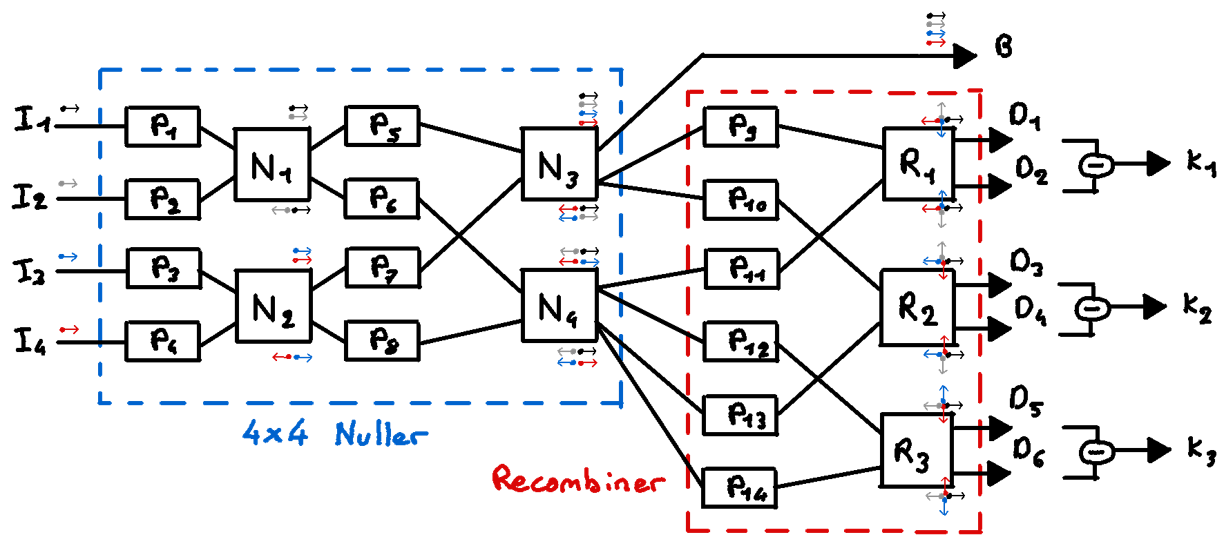
\includegraphics[width=7cm]{img/scheme.png}
            \end{tabular}
            \end{center}
            \caption[Architecture] 
            { \label{fig:architecture} 
            Scheme of our Kernel-Nuller architecture described above. The circles with colored arrows show, at different steps, the phase of each input signal we should have under ideal conditions, by taking the phase of the first input as reference. These indicators are totally fictive and there is in practice no way to know the phase of the electric field at these points. In order to limit the number of symbols used, we use $\varphi_n$ and $\sigma_n$ interchangeably to designate the elements of the phase component $e^{\mi\varphi_n}$ and $e^{\mi\sigma_n}$ introduced by the latter}
        \end{figure}
        
    %-------------------------------------------------------------------
        
    \section{System modelisation \& calibration}

        In order to study the behavior of such an active component, a numerical model of the latter was first carried out in Python \hl{[LINK TO THE REPO?]}. Given that the injection and propagation of electric fields within the component is ensured by single-mode fibers, this model describes each field via a complex amplitude and uses the first input signal phase as reference (so we always set $\varphi_1 = 0$). Thus, each operation is assimilated to a matrix acting on the complex amplitudes of these fields. In addition, although they certainly exist in practice, the coupling terms of the matrices describing the MMI are neglected because the active part of the component does not allow us to act on these phenomena anyway.
    
        In order to calibrate the component, two algorithms have been developed. The first algorithm is based on the principle of a genetic algorithm, the second one uses successive input obstruction to constrain the system and make it analytically resolvable. Both algorithms use the same principle: we seek to optimize the component's performance by introducing phase variations on each phase shifter to cancel a unique on-axis source. The difference between the two algorithms lies in the way these phase variations are introduced and in the metrics used to evaluate the performance of the component. We will present both methods and discuss their advantages and limitations.
    
        \begin{figure}[H]
            \begin{center}
            \begin{tabular}{c}
            \includegraphics[width=\linewidth]{img/phases.png}
            \end{tabular}
            \end{center}
            \caption[phases] 
            { \label{fig:phases} 
            Perturbed (a) and ideal (b) phase of each signals at the outputs of $N_1$ (top row) and $R_1$ (bottom row). By tuning the active component, the calibration process aim to get as near as possible to the ideal phase configuration. \hl{[INCREASE FONT]}}
        \end{figure}
    
        \subsection{Genetic}
            The straightforward approach is based on the principle of a deterministic genetic algorithm, which consists of successively introducing a phase variation $\Delta \phi$ in each phase shifter $\varphi_n$ and looking at how it improves or decreases the performance of the system according to some metrics.
    
            Since kernels are built using the difference of two dark outputs, it is possible to obtain very good kernel-nulls without necessarily having well nullified the star's light. In this scenario, the output signals of the cross-recombiners are not equal or in phase quadrature. A low-order aberration in the phase of one of them would cause an intensity difference on the pairs of dark outputs, and inevitably on the kernel constructed from this pair. Thus, to have robust kernels, we must ensure that the signals are perfectly in phase quadrature and therefore that the on-axis source is well canceled on the dark outputs.
            
            To address this issue, we define two different metrics, one measuring the average of kernel-null depth $M_K$ that we want to minimize, the other measuring the intensity obtained on the bright output of the component $M_B$ that we want to maximize (which, by construction, minimize the total dark output intensity).
            
            Given our component's architecture, we can associate the metric $M_B$ with each phase shifter that affects the bright output, namely $\varphi_{1 \rightarrow 5}$ and $\varphi_7$ which we will call $\vec{\varphi^{(b)}}$. All other phase shifters are then associated with the metric $M_K$ and will be called $\vec{\varphi^{(k)}}$. Thus, we are searching for the optimal phase shifts $\vec{\varphi^*} = \vec{\varphi^{(k)*}} \cup \vec{\varphi^{(b)*}}$ such as:

            \begin{equation}
                \vec{\varphi^{(b)}} = \vec{\varphi_{n \in \{1,2,3,4,5,7\}}}
            \end{equation}
            
            \begin{equation}
                \vec{\varphi^{(k)}} = \vec{\varphi_{n \in \{6,8,9,10,11,12\}}}
            \end{equation}
    
            \begin{equation}
                \vec{\varphi^{(b)*}} = \argmin_{\vec{\varphi^{(b)}}} \Big( M_B(\vec{\varphi^{(b)}}) \Big)
            \end{equation}
    
            \begin{equation}
                \vec{\varphi^{(k)*}} = \argmax_{\vec{\varphi^{(k)}}} \Big( M_K(\vec{\varphi^{(k)}}) \Big)
            \end{equation}
    
            \begin{equation}
                M_B(\vec{\varphi^{(b)}}) = |B(\vec{\varphi^{(b)}})|^2
            \end{equation}
    
            \begin{equation}
                M_K(\vec{\varphi^{(k)}}) = \frac{1}{3}\sum_{n=1}^3 |K_n(\vec{\varphi^{(k)}})|
            \end{equation}
    
            The genetic algorithm is then structured as follows.
    
            \begin{enumerate}
                \item Initialization: we initialize the phases of each phase shifter $\varphi_n$ to 0.  (cf. Algorithm \ref{genetic} line 1)
                \item Mutation: we consider two phase variations of $+ \Delta \varphi$ and $- \Delta \varphi$, successively on each phase shifter $\varphi_n$, always in the same order  (cf. Algorithm \ref{genetic} line 6-10).
                \item Selection: we retain the configuration that most improves the metric associated with that phase shifter (cf. Algorithm \ref{genetic} line 11-25). 
                \item Convergence: we repeat steps 2 and 3, reducing the value of $\Delta \varphi$ by a factor of $\beta \in [0.5,1[$ at each iteration $t$ ($\Delta \varphi(t) = \Delta \varphi(t-1) * \beta$). A factor $\beta$ close to $1$ allows for a slow but more precise convergence, whereas a $\beta$ factor of $0.5$ will yield the fastest convergence but may lead to an underoptimal solution (cf. Algorithm \ref{genetic} line 5, 27). If $\beta < 0.5$, the parameter space cannot be totally covered.
                \item Stopping point: we stop when the phase variation $\Delta \varphi$ introduced is smaller than the uncertainty in the injected phase, which must be determined through prior characterization of the phase shifters (cf. Algorithm \ref{genetic} line 5).
            \end{enumerate}
    
            \begin{algorithm}
                \caption{Straightforward approach (genetic)}
                \label{genetic}
                \SetKwInOut{Input}{Inputs}\SetKwInOut{Output}{Output}
                
                \Input{$\varepsilon$: minimal phase increment\\
                       $\beta$: phase variation reduction factor ($\beta \in [0.5,1[$)}
                \Output{$\vec{\varphi^*}$: optimized phase shifts vector}
                \BlankLine
                
                $\vec{\varphi} \leftarrow \vec{0}$ \tcp*{Initialize phase shifts to 0}
                $\Delta\varphi \leftarrow \lambda/4$ \tcp*{Initial phase variation}
                $\vec\psi = [1,1,1,1]$ \tcp*{Input signals (complex amplitude)}
                \BlankLine
                
                \While{$\Delta\varphi > \varepsilon$}{
                    \For{$n \leftarrow 1$ \KwTo $14$}{
                        $\vec{\varphi^+} \leftarrow \vec{\varphi}$\;
                        $\varphi^+_n \leftarrow \varphi_n + \Delta\varphi$\;
                        
                        $\vec{\varphi^-} \leftarrow \vec{\varphi}$\;
                        $\varphi^-_n \leftarrow \varphi_n - \Delta\varphi$\;
                        
                        \uIf{$M^{(b)}(\vec\psi, \vec{\varphi^+}) > M^{(b)}(\vec\psi, \vec{\varphi})$}{
                            $\vec{\varphi} \leftarrow \vec{\varphi^+}$\;
                            continue;
                        }
                        \If{$M^{(b)}(\vec\psi, \vec{\varphi^-}) > M^{(b)}(\vec\psi, \vec{\varphi})$}{
                            $\vec{\varphi} \leftarrow \vec{\varphi^-}$\;
                            continue;
                        }
                        
                        // We prioritize the improvement of the bright metric over the kernel one to ensure redirecting the on-axis light to the bright output
                        
                        \If{$M^{(k)}(\vec\psi, \vec{\varphi^+}) < M^{(k)}(\vec\psi, \vec{\varphi})$}{
                            $\vec{\varphi} \leftarrow \vec{\varphi^+}$\;
                            continue;
                        }
                        \If{$M^{(k)}(\vec\psi, \vec{\varphi^-}) < M^{(k)}(\vec\psi, \vec{\varphi})$}{
                            $\vec{\varphi} \leftarrow \vec{\varphi^-}$\;
                            continue;
                        }
                    }
                    $\Delta\varphi \leftarrow \beta \Delta\varphi$ \tcp*{Reduce phase variation}
                }
                \Return{$\vec{\varphi}$}
                \BlankLine
            \end{algorithm}
    
            This algorithm has the advantages of being very easy to adapt to other Kernel-Nuller architectures. In addition, it does not require any moving parts during the calibration process, allowing for fast and automated calibration. However, it suffers from two limitations. The first one is that nothing guarantees that this algorithm will converge to a global minimum/maximum on the metrics. In addition, the phase to be injected using the shifters near the outputs depends on the phase injected in the previous layers. Thus, the calibration of the final shifters can only be finely tuned once the initial shifters have been calibrated, which implies very little flux on the dark outputs during calibration and therefore a greater sensitivity to photon noise. Numerically, using a perfectly cophased Vega-like source as calibrator, it is possible to achieve kernel-null depths of the order of $10^{-8}$. \hl{[ADD LAB RESULTS]}. Moreover, this algorithm uses a factor $\beta$ to reduce the phase step at each iteration, allowing to control the speed or the precision of the algorithm. If this factor is $0.5$, the calibration algorithm will be the fastest, but it sometimes gives a subotptimal solution. As in practice there is no way to know that there is a better solution, we have to ensure the algorithm will give the best one by increasing the $\beta$ factor near to $1$, which leads to a longer calibration time.
    
        \subsection{Input obstruction}
            To overcome the limitations of the straightforward approach, another calibration method has been implemented. This method is based on the principle of obstructing the inputs of the component. We still inject an on-axis point source into the component, but this time we obstruct 2 of its inputs. We then focus on one of its outputs whose transfer function is greatly simplified, to the point of having only one parameter (phase shifter) influencing this output.
    
            The algorithm is constructed as follows:
    
            \begin{enumerate}
                \item We obstruct inputs $E_3$ and $E_4$ and then seek to maximize the bright output. Regarding the system architecture (Fig. \ref{fig:architecture}), we will then seek to optimize the null process that occurs on $N_1$. Using these simplifications, the system can then be expressed as follows:
                    
                    \begin{equation}
                        B \propto \bigg(E_1e^{\mi(\sigma_1 + \varphi_1)} + E_2e^{\mi(\sigma_2 + \varphi_2)}\bigg)e^{\mi(\sigma_5 + \varphi_5)}
                    \end{equation}
                    We don't have strict equality here due to the throughput that is not yet characterized, but is supposed constant for a given output.
                    
                    Considering that we only have access to the intensities, we are insensitive to the global phase. We can then neglect the phase factor $e^{\mi(\sigma_5 + \varphi_5)}$ and use the electric field phase of the first input as a reference phase (so we set $\varphi_1^* = 0$). Thus, the bright output intensity (starlight) can be reduced to this expression:
                    
                    \begin{equation}
                        S \propto |E_1e^{\mi\sigma_1} + E_2e^{\mi(\sigma_2 + \varphi_2)}|^2
                    \end{equation}
                    
                    We then seek a value of $\varphi_2$ that maximize $S$.
                    
                    \begin{equation}
                        \varphi_2^* = \argmax_{\varphi_2} S(\varphi_2)
                    \end{equation}
                    
                    As we add two complex numbers, we can geometrically see that $S$ can be expressed as
                    
                    \begin{equation}
                        \label{sine_function}
                        S \propto A\cos(\varphi_2 + C) + D
                    \end{equation}
                    
                    where $A = 2 \times \min(|E_1|^2, |E_2|^2)$, $D = ||E_1|^2 - |E_2|^2$ and $C = \sigma_2 - \sigma_1$. From this form, we can deduce that
                    
                    \begin{equation}
                        \varphi_2^* = - C = \sigma_1 - \sigma_2
                    \end{equation}
                    
                    This parameter $C_2$ can easily be found by fitting equation \ref{sine_function} using several measurements with different values of $\varphi_2$.
                
                \item Similarly to the first step, we obstruct $E_1$ and $E_2$ and seek to maximize $S$ by optimizing the nulling process that occurs on $N_2$. To do so, we play with $\varphi_4$ by setting $\varphi_3^* = 0$ to use this input as a reference. We then have
                    \begin{equation}
                            S \propto |E_3e^{\mi\sigma_3} + E_4e^{\mi(\sigma_4 + \varphi_4)}|^2
                    \end{equation}
                    And, using the same method, we search for
                    \begin{equation}
                        \varphi_4^* = \argmax_{\varphi_4} S(\varphi_4)
                    \end{equation}
                    We then apply the same fitting process to find the value of $\varphi_4^* = \sigma_3 - \sigma_4$
                    
                \item Once again, we obstruct $E_2$ and $E_4$ and we seek to maximize $S$. This time, the nulling operation occure on $N_3$ so we will focus on $\varphi_7$ by setting $\varphi_5^* = 0$ and using the phase of the corresponding signal as reference. The expression of the system is now a bit more complex: 
                    \begin{equation}
                        B \propto E_1e^{\mi(\sigma_1 + \varphi_1^* + \sigma_5 + \varphi_5)} + E_3e^{\mi(\sigma_3 + \varphi_3^* + \sigma_7 + \varphi_7)}
                    \end{equation}
                    In order to have only one parameter to play on, we fix $\varphi_5^* = $. We are then in the same situation as before with
                    \begin{equation}
                        S \propto |E_1e^{\mi(\sigma_1 + \sigma_5)} + E_3e^{\mi(\sigma_3 + \sigma_7 + \varphi_7)}|^2
                    \end{equation}
                    We can then fit this function and find $\varphi_7^* = \sigma_1 + \sigma_5 - \sigma_3 - \sigma_7$
                    
                \item Still obstructing $E_2$ and $E_4$, we now seek to optimize the nulling operation on $N_4$. As $N_4$ doesn't act on $S$, we will try to minimize $|D_3|^2 + |D_4|^2$ instead, which are supposed to have inputs $E_1$ and $E_3$ in perfect phase opposition. For this, we adjust phase shifter $\varphi_8$. However, minimizing a signal intensity implies to be more sensitive the different noises. A trick that we use simply consist in temporarily introducing a $\pi$ phase on $E_1$ (using delay line but it is also possible to do so by temporary modifying $\varphi_1$) and then transform the considered dark outputs into bright outputs. We then seek to maximize $|D_3|^2 + |D_4|^2$.

                    Thus, we have
    
                    \begin{equation}
                    \begin{split}
                    D_3 &\propto E_1 e^{\mi\left(\sigma_1 + \varphi_1^* + \sigma_5 + \varphi_5^* + \sigma_{10} + \varphi_{10} + \frac \pi 4\right)} \\
                        &+ E_1 e^{\mi\left(\sigma_1 + \varphi_1^* + \sigma_6 + \varphi_6^* + \sigma_{13} + \varphi_{13} - \frac \pi 4\right)} \\
                        &+ E_3e^{\mi\left(\sigma_3 + \varphi_3^* + \sigma_7 + \varphi_7^* + \frac \pi 2 + \sigma_{10} + \varphi_{10} + \frac \pi 4\right)}\\
                        &+ E_3e^{\mi\left(\sigma_3 + \varphi_3^* + \sigma_8 + \varphi_8 + \frac \pi 2 + \sigma_{13} + \varphi_{13} - \frac \pi 4\right)}\\
                    \end{split}
                    \end{equation}
    
                    \begin{equation}
                    \begin{split}
                    D_4 &\propto E_1 e^{\mi\left(\sigma_1 + \varphi_1^* + \sigma_5 + \varphi_5^* + \sigma_{10} + \varphi_{10} - \frac \pi 4\right)} \\
                        &+ E_1 e^{\mi\left(\sigma_1 + \varphi_1^* + \sigma_6 + \varphi_6^* + \sigma_{13} + \varphi_{13} + \frac \pi 4\right)} \\
                        &+ E_3e^{\mi\left(\sigma_3 + \varphi_3^* + \sigma_7 + \varphi_7^* + \frac \pi 2 + \sigma_{10} + \varphi_{10} - \frac \pi 4\right)}\\
                        &+ E_3e^{\mi\left(\sigma_3 + \varphi_3^* + \sigma_8 + \varphi_8 + \frac \pi 2 + \sigma_{13} + \varphi_{13} + \frac \pi 4\right)}\\
                    \end{split}
                    \end{equation}
    
                    At this point, we let $\varphi_{10} = \varphi_{13} = 0$ and set $\varphi_6^* = 0$ in order to use the corresponding absolute phase as reference and play on $\varphi_8$. In case we recall, we still have $\varphi_1 = \varphi_3 = \varphi_5 = 0$. The $\frac \pi 2$ terms come from the nuller MMI and the $\frac \pi 4$ comes from the cross-recombiner. By recombining all the constant terms, we thus have:
    
                    \begin{equation}
                    D_3 \propto Z e^{\mi\Phi_Z} + E_3 e^{\mi\left(\Phi + \varphi_8\right)}
                    \end{equation}
    
                    \begin{equation}
                    D_4 \propto Z' e^{\mi\Phi_{Z'}} + E_3 e^{\mi\left(\Phi' + \varphi_8\right)}
                    \end{equation}
    
                    From here, we can also geometrically see that we have
    
                    \begin{equation}
                    |D_3|^2 + |D_4|^2 \propto A'\cos(\varphi_8 + C') + D'
                    \end{equation}
    
                    Once again, we can fit this function to find $\varphi_8^*$
                
                \item At this step, we optimized all the nulling operations. It remain to optimize the cross-combination operations. To do so, we will focus on the kernel outputs and try to minimze them. We then obstruct all the inputs except $E_1$ and seek to minimize $K_1$. As a remember, $K_1$ measure the asymmetry of the signals $|D_1|^2$ and $|D_2|^2$ such as $K_1 = |D_1|^2 - |D_2|^2$. As there is only one input signal, the nulling operations will not occur and will let place to a simple beam splitters. We now set $\varphi^*_{9} = 0$ and we play on $\varphi_{11}$ to minimize $K_1$. We then have:
                
                    \begin{equation}
                        K_1 = |D_1|^2 - |D_2|^2
                    \end{equation}
                    
                    \begin{equation}
                        \begin{split}
                            K_1 & = &+ \bigg|E_1e^{\mi(\sigma_1 + \sigma_5 + \sigma_9 + \frac{\pi}{4})} + E_1e^{\mi(\sigma_1 + \sigma_6 + \sigma_{11} + \varphi_{11} - \frac{\pi}{4})}\bigg|^2 \\
                                &   &- \bigg|E_1e^{\mi(\sigma_1 + \sigma_5 + \sigma_9 - \frac{\pi}{4})} + E_1e^{\mi(\sigma_1 + \sigma_6 + \sigma_{11} + \varphi_{11} + \frac{\pi}{4})}\bigg|^2
                        \end{split}
                    \end{equation}

                    Once again, by regrouping all the constant terms and retrieve the equivalent sine function. However, this time we will not search for $\varphi_{11}$ that maximize $K_1$, but that cancel it (or alternatively, search the value that minimize the absolute value of $K_1$). By fitting the sine function, it is trivial to get $\varphi^*_{11}$. There is actually two solutions that are equivalent.

                    \item We repeat the latter operation by looking at $K_2$, fixing $\varphi_{10}$ and playing on $\varphi_{13}$ to find $\varphi^*_{13}$.

                    \item We finally do the same operation one last time, looking at $K_3$, fixing $\varphi_{12}$ and playing on $\varphi_{14}$ to find $\varphi^*_{14}$.
                
            \end{enumerate}
    
            This second calibration method has the advantage of not suffering from photon-noise sensitivity since we ensure at each step that we have flux on the outputs of interest. However, it is adapted to our architecture and must be completely rethought to be adapted to another Kernel-Nuller architecture. Moreover, it requires the action of moving parts to obstruct the component's input, which can be a disadvantage for automated calibration.
    
            Using this method, we are numerically able to obtain very deep null depth, proportionally to the number of measurements taken for each fitting process. \hl{[ADD LAB RESULTS]}
    
            \begin{algorithm}
                \caption{Obstruction approach}
                \label{obstruction}
                \SetKwInOut{Input}{Inputs}\SetKwInOut{Output}{Output}
                
                \Input{$N$: phase resolution}
                \Output{$\vec{\varphi}$: optimized phase shifts vector}
                \BlankLine
                
                $\vec{\varphi}^* \leftarrow \vec{0}$ \tcp*{Initialize phase shifts to 0}
                \BlankLine
                $\vec{\psi} = [1, 1, 0, 0]$ \tcp*{Input signals (complex amplitude)}
                $\varphi_2^* = \argmax_{\varphi_2}S(\vec\psi, \varphi_2)$\;
                \BlankLine
                $\vec{\psi} = [0, 0, 1, 1]$\;
                $\varphi_4^* = \argmax_{\varphi_4}S(\vec\psi, \varphi_4)$\;
                \BlankLine
                $\vec{\psi} = [0, 1, 0, 1]$\;
                $\varphi_7^* = \argmax_{\varphi_7}S(\vec\psi, \varphi_7)$\;
                \BlankLine
                $\vec{\psi} = [1, 0, -1, 0]$\;
                $\varphi_8^* = \argmax_{\varphi_8}|D_1(\vec\psi, \varphi_8)|^2 + |D_2(\vec\psi, \varphi_8)|^2$\;
                \BlankLine
                $\vec{\psi} = [1, 0, 0, 0]$\;
                $\varphi_{11}^* = \argmin_{\varphi_{11}}\left|K_1(\vec\psi, \varphi_{11})\right|$\;
                $\varphi_{13}^* = \argmin_{\varphi_{13}}\left|K_2(\vec\psi, \varphi_{13})\right|$\;
                $\varphi_{14}^* = \argmin_{\varphi_{14}}\left|K_3(\vec\psi, \varphi_{14})\right|$\;
                
                \Return{$\vec{\varphi}^*$}
                \BlankLine
            \end{algorithm}
    
    %--------------------------------------------------------------------
    
    \section{Results and limitations}

        \subsection{Numerical results}

            

            \begin{figure}
                \begin{center}
                \begin{tabular}{c}
                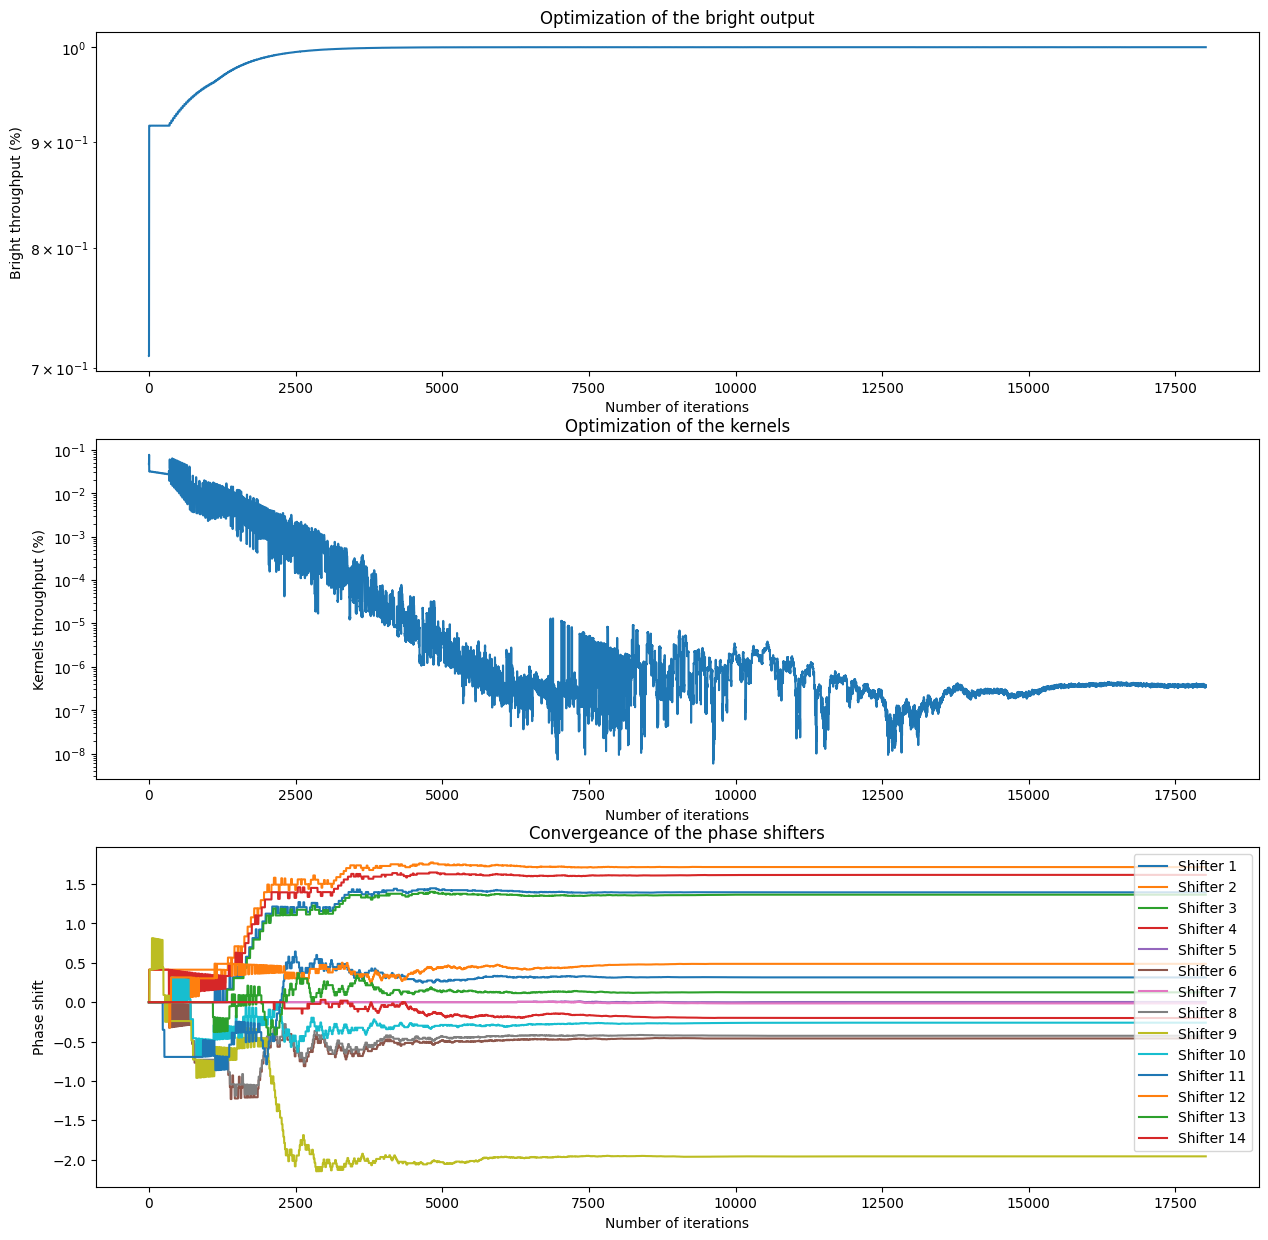
\includegraphics[width=\linewidth]{img/calibration_genetic.png}
                \end{tabular}
                \end{center}
                \caption[Calibration Genetic] 
                { \label{fig:calibration_genetic} 
                Evolution of the performances and the state of the phase shifters during the calibration process via the genetic approach. On the top plot, we see the progressive increase of the flux on the bright output as well as, on the middle plot, the progressive decrease of the flux on the kernel outputs (sum of the absolute values of the three kernels). The light intensities at the outputs are reported to that introduced in the inputs, i.e. the throughput of the system. On the bottom plot, we see the evolution of the phase introduced on each phase shifter. \hl{[INCREASE FONT]}}
            \end{figure}
    
            \begin{figure}
                \begin{center}
                \begin{tabular}{c}
                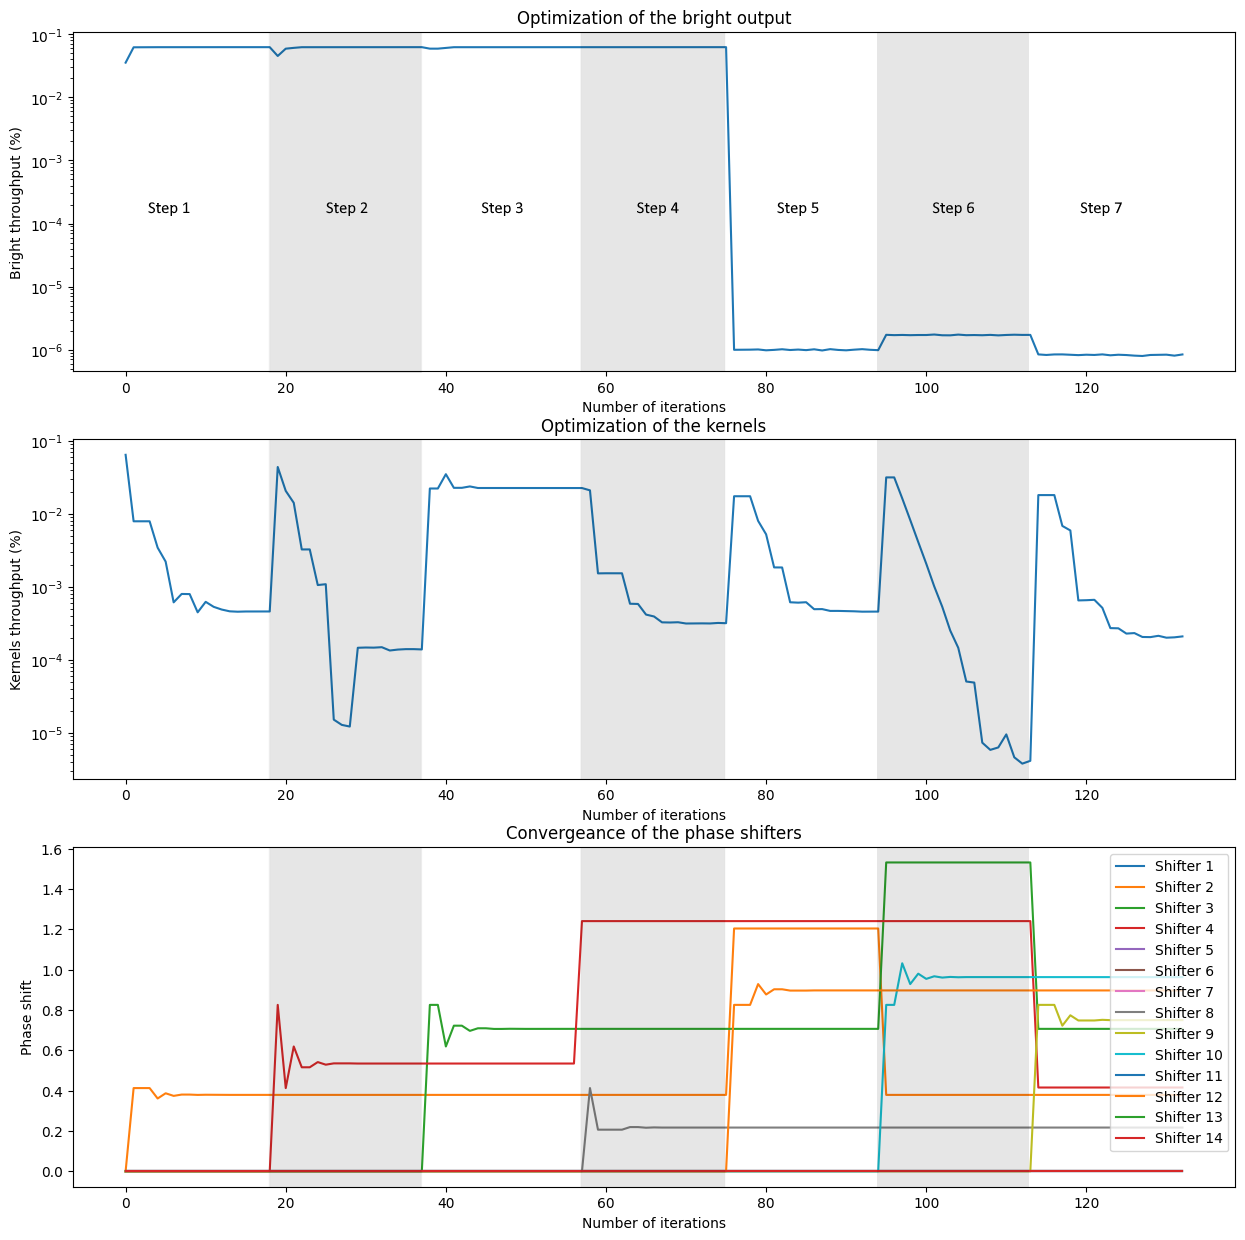
\includegraphics[width=\linewidth]{img/calibration_obstruction.png}
                \end{tabular}
                \end{center}
                \caption[calibration obstruction] 
                { \label{fig:calibration_obstruction} 
                Fitting of each transfer function once the system is reduced to one degree of freedom. \hl{[INCREASE FONT]}}
            \end{figure}

            \begin{figure}
                \begin{center}
                \begin{tabular}{c}
                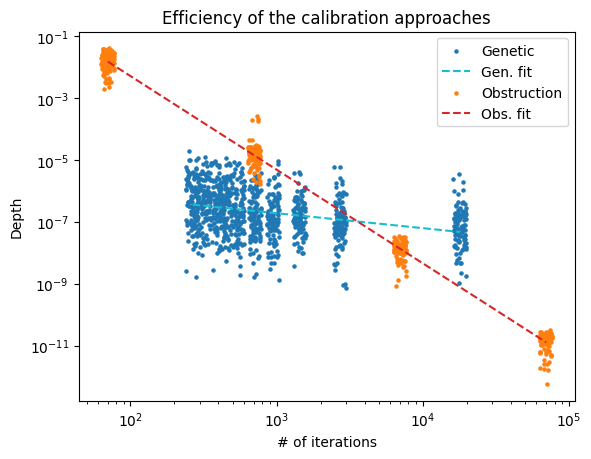
\includegraphics[width=\linewidth]{img/method_comparison.png}
                \end{tabular}
                \end{center}
                \caption[method comparison] 
                { \label{fig:method_comparison} 
                Average kernel-Null depth as function of the number of calibration steps in both genetic and obstruction-based algorithms. \hl{[INCREASE FONT]}}
            \end{figure}
        
        \subsection{Laboratory results}

        \subsection{Laboratory limitations}
    
        \begin{figure}
            \begin{center}
            \begin{tabular}{c}
            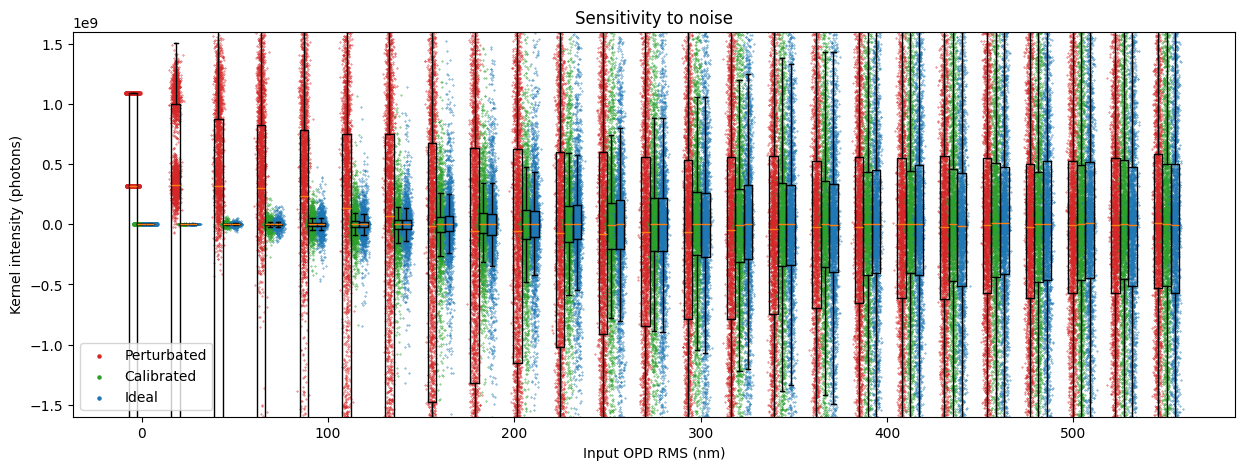
\includegraphics[width=\linewidth]{img/noise_sensitivity.png}
            \end{tabular}
            \end{center}
            \caption[noise sensitivity] 
            { \label{fig:noise_sensitivity} 
            \hl{[TO DO]} \hl{[INCREASE FONT]}}
        \end{figure}
    
    %-----------------------------------------------------------------
    
    \section{Conclusions and prospects}
    
       \begin{enumerate}
          \item Conditions for noticing a performance gain
          \item Need of a post calibration characterization process to identify the outputs
          \item Deeper statistical analysis is required to truly characterize performance gain (the null depth is not the only relevant parameter)
          \item Architecture limitations (ex. no amplitude modulation, no photometric outputs, mono-chromaticity)
       \end{enumerate}
    
    \begin{acknowledgements}
          Lorem ipsum
    \end{acknowledgements}
    
    % WARNING
    %-------------------------------------------------------------------
    % Please note that we have included the references to the file aa.dem in
    % order to compile it, but we ask you to:
    %
    % - use BibTeX with the regular commands:
    %   \bibliographystyle{aa} % style aa.bst
    %   \bibliography{Yourfile} % your references Yourfile.bib
    %
    % - join the .bib files when you upload your source files
    %-------------------------------------------------------------------
    
    \bibliographystyle{aa} % We choose the "plain" reference style
    \bibliography{refs} % Entries are in the refs.bib file

\end{document}
